\documentclass{scrreprt}
\usepackage{graphicx}
\usepackage[utf8]{inputenc}
\usepackage{tikz}
\usepackage{listings}
\usepackage{underscore}
\usepackage[bookmarks=true]{hyperref}
\usepackage[section]{placeins}
\hypersetup{
    bookmarks=false,    % show bookmarks bar?
    pdftitle={Software Requirement Specification},    % title
    pdfauthor={Yiannis Lazarides},                     % author
    pdfsubject={TeX and LaTeX},                        % subject of the document
    pdfkeywords={TeX, LaTeX, graphics, images}, % list of keywords
    colorlinks=true,       % false: boxed links; true: colored links
    linkcolor=blue,       % color of internal links
    citecolor=black,       % color of links to bibliography
    filecolor=black,        % color of file links
    urlcolor=purple,        % color of external links
    linktoc=page            % only page is linked
}%
\def\myversion{1.0}
\date{}
\usepackage{hyperref}
\begin{document}
\begin{titlepage}
  \flushright\bfseries\huge
  \vspace*{\stretch{0.4}}
    \rule{\linewidth}{5pt}
    \par
    \vspace{1cm}
    {\Huge DESIGN \par DOCUMENT \par}
    \vspace{2cm}
    for \\
    \vspace{2cm}
    Personal Dietary Application \\
    \vspace{2cm}
     \LARGE{Version \myversion \\}
    \vspace{2cm}
    by Craig Boucher \\
    Md Tanveer Alamgir \\
    Fan \\
    Osman \\
    Xin
    \vspace{2cm}
    \rule{\linewidth}{5pt}
    \vspace{\stretch{1}}
\end{titlepage}
\tableofcontents
\chapter{Introduction}
The project undertaken in this COMP 5541 course involves creating an application that keeps track of dietary records for the user. This diet app has been designed to use the border pane layout for the main window. \\ \\ 
This design document will provide details for the type of software architecture used to develop the software and explain the design for the user interface. The architectural component illustrates the abstraction of the software classes involved and how they relate to each other to maniuplate and process data that the user interacts with. The interface design section will assess the process for the states the user goes through to interact with the personal dietary application.
\section{Purpose}
This document will serve as an illustration for the architectural design choices as well as an explanation for the properties of the user interface implemented for the Personal Dietary Application software. This software project is being completed for the COMP 5541 graduate diploma course at Concordia University. There will be diagrams to chowcase the type of the architecture used and a class diagram. Screenshots are used to provide a valuable perspective on the user interface. These graphical aids are described in further detail to demonstrate the functionality of the interface.
\section{Scope}
In order to provide proper design documentation for the Personal Dietary Application this document will be properly formatted and included all necessary information. The team responsible for surveying this document and creating the software will be able to use the robust explanation of the architectural model presented in this document to carry out the necessary work. The visual graphics demonstrating the user interface design choices will serve as a guide for the team to orchestrate the proper performance of the software.
\section{Definitions and Abbreviations}
\subsection{Definitions}
\begin{tabular}{|l|l|}
\hline
	Term & Definition \\
\hline
	Model View & Software architecture that renders funcionality between three components. \\
	Controller & The view is the user interface. The model stores the data and the controller \\
	& mediates data transfer between the view and model. \\
\hline
	Date & Allows user to enter day and month of an entry for an item. \\
\hline
	Consumed & The user will be able to mark a food item as consumed (eaten) or not. \\
\hline
\end{tabular}

\subsection{Abbreviations}
\begin{tabular}{|l|l|}
\hline
	Abbreviation & Term \\
\hline
	MVC & Model View Controller \\
\hline
	GUI & Graphical User Interface \\
\hline
	UML & Unified Modeling Language \\
\hline
	PDA & Personal Dietary Application \\
\hline
\end{tabular}

\section{References}
https://upload.wikimedia.org/wikipedia/commons/a/a0/MVC-Process.svg \\
http://users.encs.concordia.ca/~paquet/wiki/images/e/ee/Phase2final.pdf
\section{Overview}
The rest of the document is composed of two main sections. First, there is a section dedication to Architectural Design. Lastly, the largest section, consists of Software Interface Design. In the portion concerning the software architecture the three smaller sections are related to the reasoning for choosing the architecture, a diagram illustrating how the architecture behaves abstractly, and the final section details how software files will operate together on the computer. \\
The interface section will provide documentation regarding the system, modules, and dynamic interfaces for the software project.
\chapter{Architectural Design}
\section{Rationale}
The Model View Controller (MVC) architecture design pattern has been chosen for this software project. Model, View, and Controller are the three components which comprise this architecture. \\

The purpose of the Controller model is to navigate and facilitate the transfer of data between the View and the Model. The Controller is responsible for acquiring data input from the user, manipulate the model with the necessary memory changes, and potentially provide updates to the View if and when exceptions or errors are thrown. \\

The View is where the (graphical) user interface rests. The information stored in the model is used by the View to display everything necessary to the user. Everything the user interacts with rests with the View, from input functionality to button objects. Whenever data is manipulated in the Model the View will reflect this accordingly. \\

The objective of the Model is to store all of the necessary information and data that the application requires to operate successfully. All of the data is stored in local memory. Every food item and all of the details of each item is stored in the Model module. There is a list of every food item added by the user that is stored in the Model, and whenever a change is made (adding or removing food items), the View will graphically respond to these changes. \\

\begin{center}
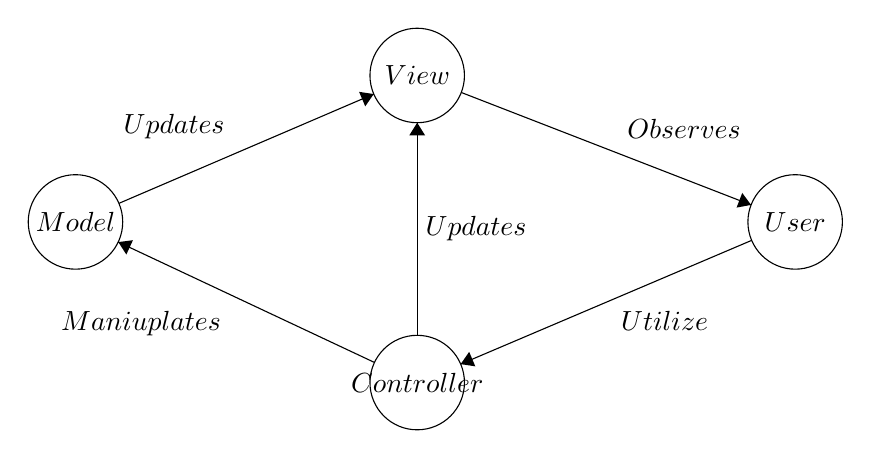
\begin{tikzpicture}[scale=0.2]
\tikzstyle{every node}+=[inner sep=0pt]
\draw [black] (39.5,-15.1) circle (3);
\draw (39.5,-15.1) node {$View$};
\draw [black] (17.8,-24.4) circle (3);
\draw (17.8,-24.4) node {$Model$};
\draw [black] (39.5,-34.6) circle (3);
\draw (39.5,-34.6) node {$Controller$};
\draw [black] (63.5,-24.4) circle (3);
\draw (63.5,-24.4) node {$User$};
\draw [black] (42.3,-16.18) -- (60.7,-23.32);
\fill [black] (60.7,-23.32) -- (60.14,-22.56) -- (59.78,-23.49);
\draw (56.44,-19.14) node [above] {$Observes$};
\draw [black] (60.74,-25.57) -- (42.26,-33.43);
\fill [black] (42.26,-33.43) -- (43.19,-33.57) -- (42.8,-32.65);
\draw (55.21,-30.05) node [below] {$Utilize$};
\draw [black] (36.78,-33.32) -- (20.52,-25.68);
\fill [black] (20.52,-25.68) -- (21.03,-26.47) -- (21.45,-25.56);
\draw (21.96,-30.05) node [below] {$Maniuplates$};
\draw [black] (20.56,-23.22) -- (36.74,-16.28);
\fill [black] (36.74,-16.28) -- (35.81,-16.14) -- (36.2,-17.06);
\draw (24.06,-19.19) node [above] {$Updates$};
\draw [black] (39.5,-31.6) -- (39.5,-18.1);
\fill [black] (39.5,-18.1) -- (39,-18.9) -- (40,-18.9);
\draw (40,-24.85) node [right] {$Updates$};
\end{tikzpicture}
\end{center}

The software specifications outlined in the project instructions specifically mandated the MVC architecture. The purpose of this architecture is to provide a relevant abstraction of how desktop, mobile, or web applications operate when requiring constant use by a user. The abstraction allows three distinct modules to operate independently of each other and be capable of being updated separately. Different developers can be assigned to develop for the various modules with minimal cooperation required between them as the core functionality of each module remains the same across updates.

\section{Software Architecture Diagram}
\includegraphics[height=9cm]{MVC-Process.png}
\section{System Topology}
\chapter{Software Interface Design}
\section{System Interface Diagrams}

Our personal dietary application has only system level interface. The application does not employ any software or hardware interfaces. GUI is the system level interface. GUI allows the user to interact with the application. Using GUI user will be able to add a food item, mark it as eaten or not eaten, hide an added item, remove an item and the update of the dietary.

\subsection{User Interface}

User will interact with the computer using the user interface. We tried to make it as user friendly as possible by placing the components with an order of their importance and utilizing the full screen mode. Below are the few points we took into consideration for user interface:

\begin{itemize}
	\item User Friendly: Making it user friendly by putting important components according to user's view point.
	\item Easy to find information: Since the application is all about their dietary, so it was important to make it easy to calculate and display their consumed and need to consumed items. We make it as handy as possible.
	\item Guiding user: Guiding user by displaying different colour if they miss out something while inputting a food item.
\end{itemize}

\section{Dynamic Models of System Interface}
The system interfaces that establish the interaction between user and computer are described below:
\clearpage
\subsection{Add Food Item Scenario}

	\begin{figure}[h]
	\centering
	\includegraphics[width=15cm]{pictures/raw.png}
	\caption{Adding a food item scenario}
	\end{figure}


\subsection{Remove Food Item Scenario}
\subsection{Set Food Item as Consumed Scenario}
\subsection{Set Food Item as Unconsumed Scenario}
\subsection{Hide Consumed Diet Scenario}
\subsection{Unhide Consumed Diet Scenario}

\section{Module Interface Diagrams}
\begin{center}
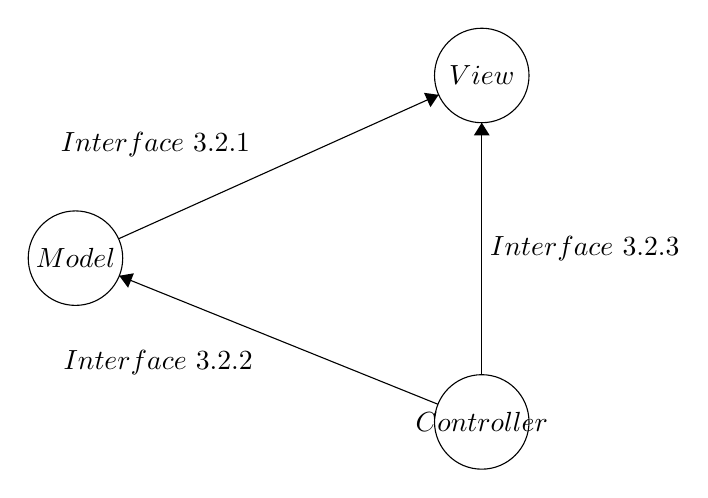
\begin{tikzpicture}[scale=0.2]
\tikzstyle{every node}+=[inner sep=0pt]
\draw [black] (39.5,-15.1) circle (3);
\draw (39.5,-15.1) node {$View$};
\draw [black] (13.7,-26.7) circle (3);
\draw (13.7,-26.7) node {$Model$};
\draw [black] (39.5,-37.1) circle (3);
\draw (39.5,-37.1) node {$Controller$};
\draw [black] (36.72,-35.98) -- (16.48,-27.82);
\fill [black] (16.48,-27.82) -- (17.04,-28.58) -- (17.41,-27.66);
\draw (18.95,-32.54) node [below] {$Interface\mbox{ }3.2.2$};
\draw [black] (16.44,-25.47) -- (36.76,-16.33);
\fill [black] (36.76,-16.33) -- (35.83,-16.2) -- (36.24,-17.11);
\draw (18.78,-20.32) node [above] {$Interface\mbox{ }3.2.1$};
\draw [black] (39.5,-34.1) -- (39.5,-18.1);
\fill [black] (39.5,-18.1) -- (39,-18.9) -- (40,-18.9);
\draw (40,-26.1) node [right] {$Interface\mbox{ }3.2.3$};
\end{tikzpicture}
\end{center}
\subsection{View Interface}
\subsubsection{FXApp}
\subsubsection{FXController}
\subsubsection{DiningTableRow}
\subsection{Model Interface}
\subsection{Controller Interface}

% add other chapters and sections to suit
\end{document}
